\documentclass[
% handout,
center,
% aspectratio=169
]{beamer}

\usepackage[utf8]{inputenc}
\usepackage[english]{babel}
\usepackage{cite}
\usepackage{amsmath,amssymb,amsfonts}
\usepackage[linesnumbered,ruled,vlined]{algorithm2e}
\usepackage[noabbrev,capitalize]{cleveref}
\usepackage{array, booktabs, makecell}
\usepackage{graphicx}
\usepackage{textcomp}
\usepackage{xcolor}
\usepackage{caption}
\usepackage{subcaption}
\usepackage{diagbox}
\usepackage{tikz}
\usepackage{soul}
\DontPrintSemicolon

\title[Huffman Coding]{\textsc{Huffman Coding}}
\author[Bozzo - Yin]{Francesco Bozzo \and Michele Yin}
\institute[UniTN]{University of Trento}
\date{December 15, 2022}

% \logo{\includegraphics[height=1.5cm]{logo.png}}
%\usetheme{Madrid}
\definecolor{links}{HTML}{54489a}
\hypersetup{colorlinks,linkcolor=,urlcolor=links}
\usetheme{metropolis}
\setbeamercolor{background canvas}{bg=white}

\begin{document}

\begin{frame}
\titlepage
\end{frame}

% table of contents
% \AtBeginSection[]
% {
%     \begin{frame}{Table of Contents}
%         \begin{columns}[t]
%             \column{.45\textwidth}
%             \tableofcontents[sections=1-2, currentsection]

%             \column{.45\textwidth}
%             \tableofcontents[sections=3-5, currentsection]
%         \end{columns}
%     \end{frame}
% }

\section{Introduction}

\begin{frame}{Introduction}
    Table of contents
    \begin{itemize}
        \item The Huffman Coding Algorithm
        \item Serial Implementation
        \item Parallel Implementation
        \item Performance Evaluation and Benchmarks
        \item Q\&A
    \end{itemize}
\end{frame}

\begin{frame}{The Huffman Coding Algorithm}
    Huffman Coding is a \textbf{lossless data compression} algorithm  designed to find a more convenient bit representation to store data through variable-length sequences of bits defined as \emph{alphabet}.
    \begin{table}[]
        \centering
        \begin{tabular}{lll}
            \toprule
            ASCII character & Byte encoding & Huffman encoding \\
            \midrule
             a &  01100001 & 00 \\
             b &  01100010 & 010 \\
             c &  01100011 & 011 \\
             d &  01100100 & 10 \\
             e &  01100100 & 11 \\
             \bottomrule
        \end{tabular}
        \caption{Example of Huffman alphabet for 5 letters}
        \label{tab:my_label}
    \end{table}
\end{frame}

\begin{frame}{Frequency-based Encoding}
    The Huffman code for each character is decided by the occurrences of that character in the text using a \textbf{greedy} procedure:
    \begin{itemize}
        \item more frequent -> less bits
        \item less frequent -> more bits
    \end{itemize}
\end{frame}

\begin{frame}{Optimal Prefix Code}
    Even if the the Huffman algorithm is based on a greedy approach, it is able to generate an \textbf{optimal prefix code} in space efficiency.
\end{frame}

\section{Serial Version}

\begin{frame}{Serial Version}
    The Huffman Compression Algorithm is composed by four phases:
    \begin{enumerate}
        \item Count the byte frequencies
        \item Build the Huffman tree using the frequencies
        \item Generate the Huffman alphabet by visiting the Huffman tree by using a DFS algorithm
        \item Data encoding using the Huffman alphabet
    \end{enumerate}
\end{frame}

\begin{frame}{Build the Huffman Tree}
    \centering
    \scalebox{.8}{
        \begin{algorithm}[H]
            \caption{Build the Huffman tree}\label{alg:buildtree}
            \SetKwData{Q}{Q}\SetKwData{z1}{z1}\SetKwData{z2}{z2}\SetKwData{z}{z}
            \SetKwFunction{insert}{insert}\SetKwFunction{deleteMin}{deleteMin}
            \SetKwInOut{Input}{input}\SetKwInOut{Output}{output}
            \SetKwFor{}{}{}{}
            // Populate the min priority queue with characters and their frequencies\;
            \For{\(i=1\) \KwTo \(n-1\)}{
                Q.insert(f[i], Tree(f[i], c[i]))\;
            }
            // Repeat until the queue has only a single element left\;
            \For{\(i=1\) \KwTo \(n-1\)}{
                // Get the two least frequent nodes\;
                z1, z2 = Q.deleteMin(), Q.deleteMin()\;
                // Create and insert inner tree node into the queue\;
                z = Tree(z1.f + z2.f, null)\;
                z.left, z.right = z1, z2\;
                Q.insert(z.f, z)\;
            }
            // The last element in the queue is the root of the Huffman tree\;
            \Return{Q.deleteMin()}\;
        \end{algorithm}
    }
\end{frame}

\begin{frame}{Get the Huffman Alphabet from the Tree}
    Make a DFS visit of the Tree from root to leaves
    \begin{center}
        \begin{figure}[h!]
            \centering
            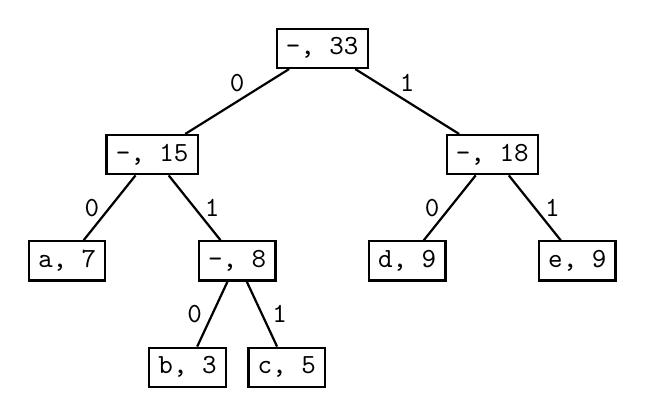
\begin{tikzpicture}
                [
                    level distance=1.5cm,
                    level 1/.style={sibling distance=4.8cm},
                    level 2/.style={sibling distance=2.4cm},
                    level 3/.style={sibling distance=1.4cm},
                    thick,
                    font=\ttfamily\bfseries, scale=0.9
                ]
                \tikzset{
                    treenode/.style = {rectangle, draw=black, align=center,minimum width=0.75cm},
                    edgestyleL/.style = {midway,left,draw=none},
                    edgestyleR/.style = {midway,right,draw=none}
                }
                \node [treenode] (T) {-, 33}
                child { node[treenode] (L) {-, 15}
                        child { node[treenode] (LL) {a, 7} edge from parent node[edgestyleL] {0} }
                        child { node[treenode] (LR) {-, 8}
                                child { node[treenode] (LRL) {b, 3} edge from parent node[edgestyleL] {0} }
                                child { node[treenode] (LRR) {c, 5} edge from parent node[edgestyleR] {1} }
                                edge from parent node[edgestyleR] {1}
                            }
                        edge from parent node[edgestyleL,above] {0}
                    }
                child { node[treenode] (R) {-, 18}
                        child { node[treenode] {d, 9} edge from parent node[edgestyleL] {0}}
                        child { node[treenode] {e, 9} edge from parent node[edgestyleR] {1}}
                        edge from parent node[edgestyleR,above] {1}
                    }
                ;
            \end{tikzpicture}
            \caption{An example of Huffman tree.}
            \label{fig:tree}
        \end{figure}
    \end{center}
\end{frame}



\section{Parallelization}
\begin{frame}{\st{Serial} Parallel Version}
    The Huffman Compression Algorithm is composed by four phases:
    \begin{enumerate}
        \item \textbf{Count} the byte frequencies
        \item Build the Huffman tree using the frequencies
        \item Generate the Huffman alphabet by visiting the Huffman tree by using a DFS algorithm
        \item \textbf{Data encoding} using the Huffman alphabet
    \end{enumerate}
    Step 1 and 4 are the most expensive and easiest to parallelize
\end{frame}
\begin{frame}{Parallelization}
    \begin{itemize}
        \item Multiple \textbf{processes} should handle separate files.
        \item Multiple \textbf{threads} of the same process should work on different chunks of the same file in parallel.
    \end{itemize}
\end{frame}
\begin{frame}{Reasoning}
    \begin{itemize}
        \item In most operating systems a file is a resource that the OS gives to a single process to avoid I/O race conditions.
        \item Because threads of the same process share the address space, we can avoid the expensive data transfer across processes.
    \end{itemize}
\end{frame}

\begin{frame}{Multithreading}
    Given $m$ threads:

    \begin{enumerate}
        \item A file is divided into $c$ \emph{chunks}, usually $m < c$ 
        \item Until all chunks are not processed:
        \begin{enumerate}
            \item A single thread reads $m$ chunks and stores them in a shared memory space
            \item Each thread works on its own assigned chunk
            \item A single thread writes the processed chunks on the disk
        \end{enumerate}
    \end{enumerate}
\end{frame}

\begin{frame}{Architecture}
    \begin{figure}
        \centering
        \includegraphics[width=\linewidth]{../imgs/threading}
        \caption{Simple schema for processing a single file with multiple threads.}
        \label{fig:threading}
    \end{figure}
\end{frame}
  \begin{frame}{Multiprocessing}
    \begin{itemize}
        \item Rank 0 gathers all files in the input folder
        \item Reads their size
        \item Distributes to other processes files, balancing the load using a min priority Q
        \item Each process work on its own queue of jobs 
    \end{itemize}
\end{frame}
    \begin{frame}{Multiprocess Architecture}
    \begin{figure}
        \centering
        \includegraphics[width=0.40\textwidth]{../imgs/overall flow schema.png}
        \caption{Simple overall schema}
        \label{fig:threading}
    \end{figure}
\end{frame}
\begin{frame}{Implementation notes}
    \begin{itemize}
        \item 1 byte as alphabet. More bytes results in less collisions and therefore less efficiency
        \item 4096 B as chunk size, because it is the standard linux page size
        %\item I/O is not real I/O, but is a request to the OS to do the I/O
    \end{itemize}
\end{frame} 

\begin{frame}{Alternative Architecture (with Locks)}
    \begin{figure}
        \centering
        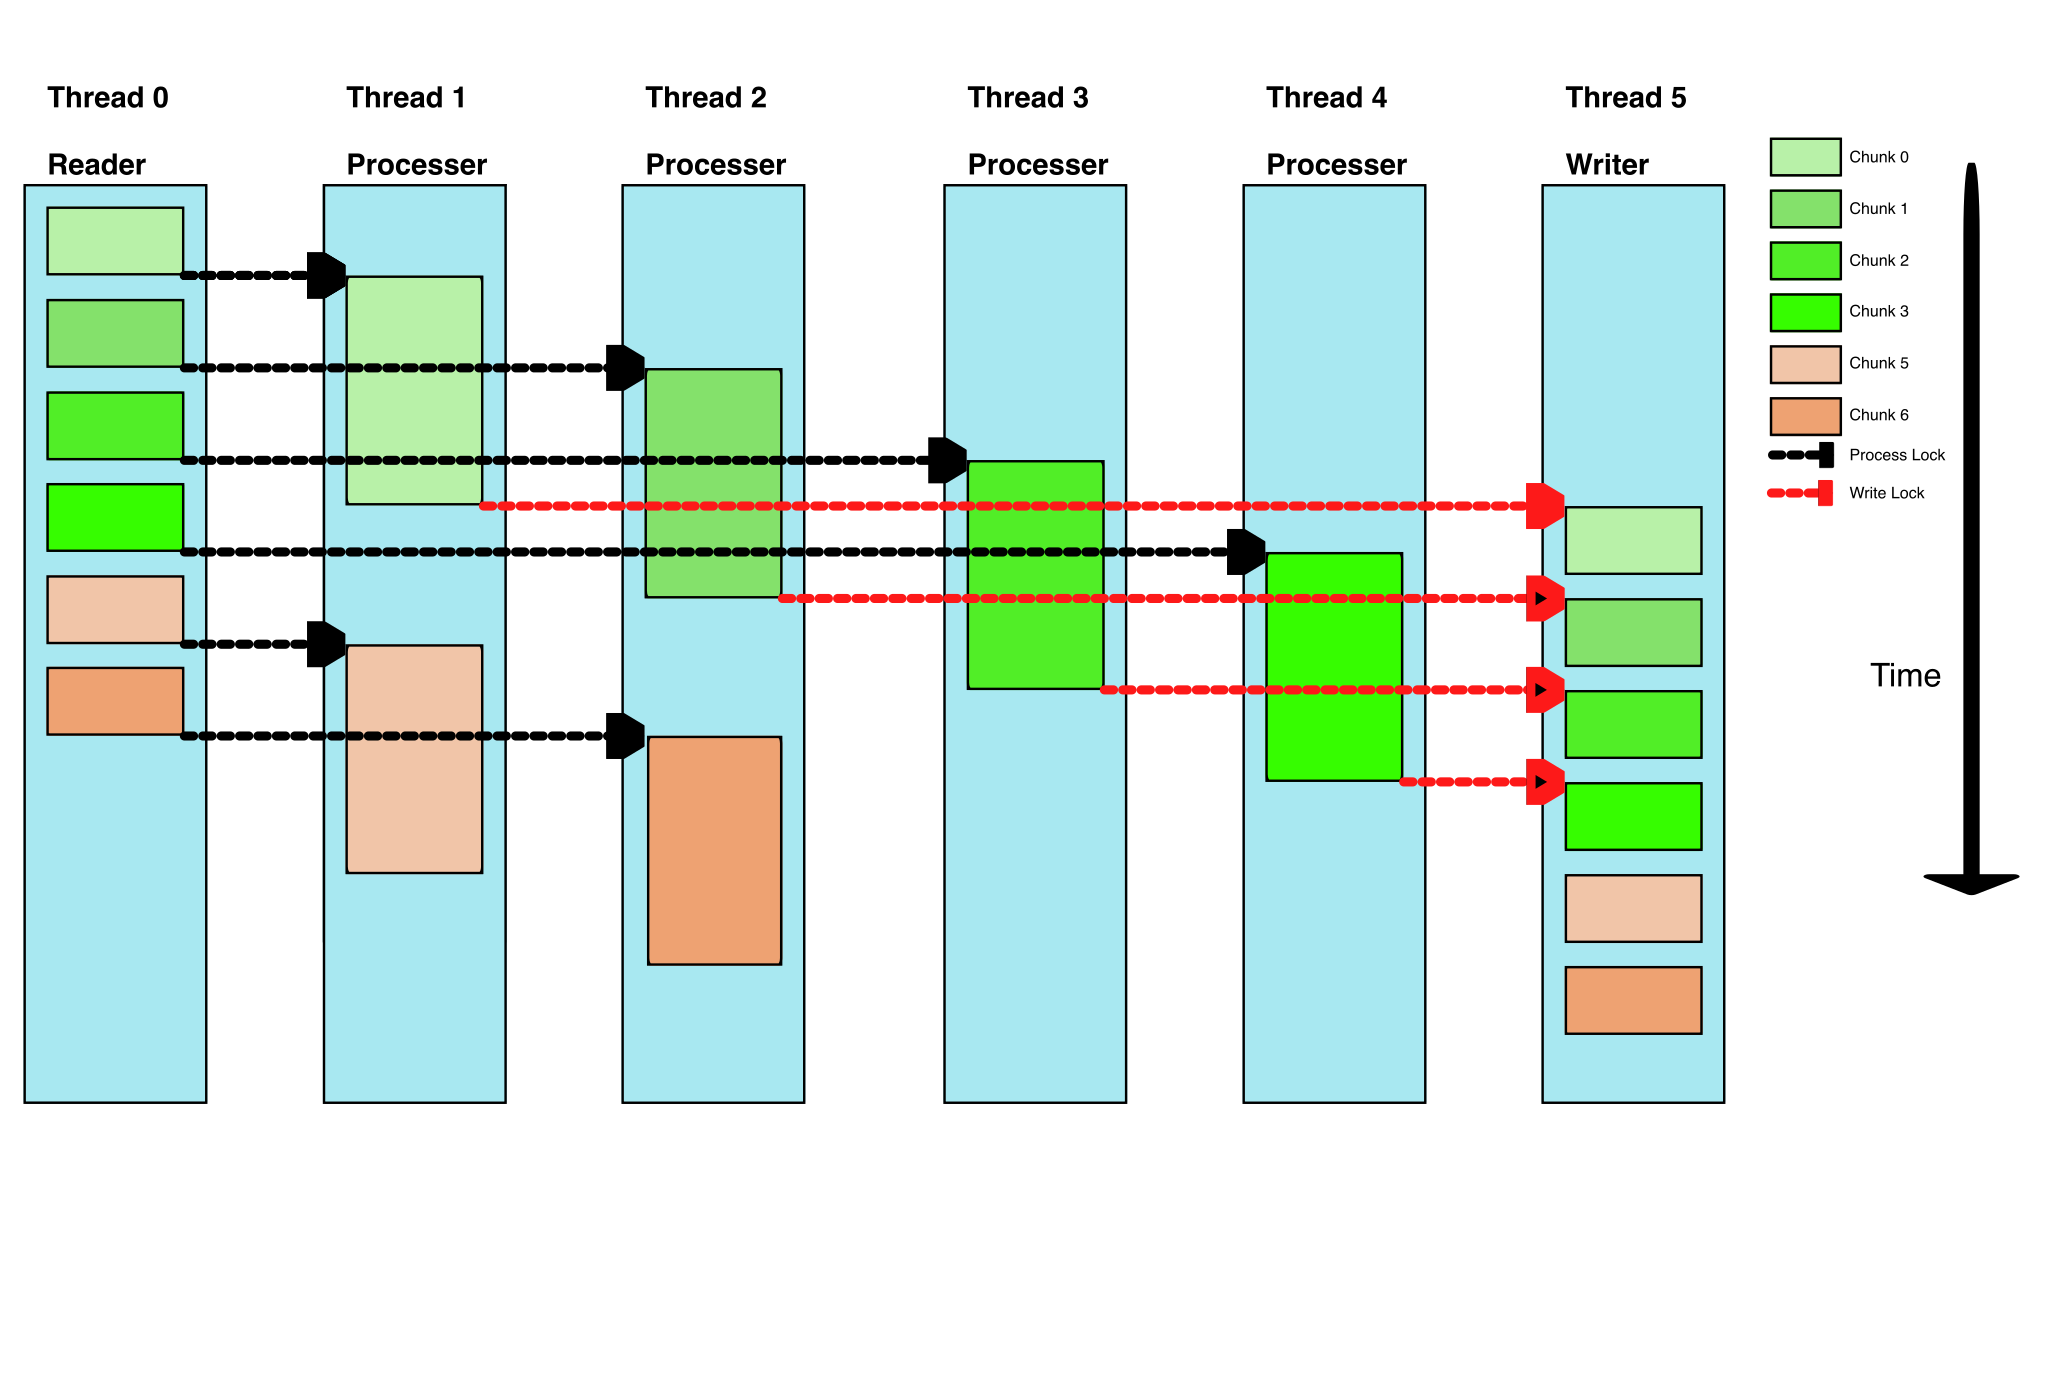
\includegraphics[width=\linewidth]{../imgs/dedicated IO threads}
        \caption{Simple schema for processing a multiple files.}
        \label{fig:threading}
    \end{figure}
\end{frame}

\section{Performance and Results}
% \begin{frame}{Results}
%     \begin{columns}
%         \column{0.5\textwidth}
%             \begin{figure}
%                 \centering
%                 \includegraphics[width=\textwidth]{imgs/encoding average speedup.png}
%                 \caption{Encoding speedup vs flush}
%                 \label{fig:encoding-speedup-vs-flush}
%             \end{figure}
%         \column{0.5\textwidth}
%             \begin{figure}
%                 \centering
%                 \includegraphics[width=\textwidth]{imgs/decoding average speedup.png}
%                 \caption{Decoding speedup vs flush}
%                 \label{fig:decoding-speedup-vs-flush}
%             \end{figure}
%     \end{columns}
% \end{frame}

\begin{frame}{Results - Encoding}
    \begin{columns}
        \column{0.5\textwidth}
            \begin{figure}
                \centering
                \includegraphics[width=\textwidth]{imgs/encoding speedup.png}
                \caption{Encoding speedup}
                \label{fig:encoding-speedup}
            \end{figure}
        \column{0.5\textwidth}
            \begin{figure}
                \centering
                \includegraphics[width=\textwidth]{imgs/encode efficiency.png}
                \caption{Encoding efficiency}
                \label{fig:encoding-efficiency}
            \end{figure}
    \end{columns}
\end{frame}
\begin{frame}{Results - Decoding}
    \begin{columns}
        \column{0.5\textwidth}
            \begin{figure}
                \centering
                \includegraphics[width=\textwidth]{imgs/decode speedup.png}
                \caption{Decoding speedup}
                \label{fig:encoding-speedup}
            \end{figure}
        \column{0.5\textwidth}
            \begin{figure}
                \centering
                \includegraphics[width=\textwidth]{imgs/decode efficiency.png}
                \caption{Decoding efficiency}
                \label{fig:encoding-efficiency}
            \end{figure}
    \end{columns}
\end{frame}
\begin{frame}{Results - Barrier vs Locks}
    \begin{columns}
        \column{0.5\textwidth}
            \begin{figure}
                \centering
                \includegraphics[width=\textwidth]{imgs/encode average speedup barrier vs locks.png}
                \caption{Encoding speedup barrier vs locks}
                \label{fig:encoding-speedup}
            \end{figure}
        \column{0.5\textwidth}
            \begin{figure}
                \centering
                \includegraphics[width=\textwidth]{imgs/decode average speedup barrier vs locks}
                \caption{Decoding speedup barrier vs locks}
                \label{fig:encoding-efficiency}
            \end{figure}
    \end{columns}
\end{frame}
\begin{frame}{Results - Ours vs Online Implementation}
    \begin{columns}
        \column{0.5\textwidth}
            \begin{figure}
                \centering
                \includegraphics[width=\textwidth]{imgs/average ours vs 7}
                \caption{Average encoding speedup ours vs online 7}
                \label{fig:encoding-speedup}
            \end{figure}
        \column{0.5\textwidth}
            \begin{figure}
                \centering
                \includegraphics[width=\textwidth]{imgs/ours vs online 7 1-500}
                \caption{Encoding speedup ours vs online 7}
                \label{fig:encoding-efficiency}
            \end{figure}
    \end{columns}
\end{frame}
\begin{frame}{Results - Folders}

        \begin{figure}
            \centering
            \includegraphics[width=\textwidth]{imgs/linux speedup.png}
            \caption{Encoding speedup with Linux}
            \label{fig:encoding-linux}
        \end{figure}
\end{frame}


% \include{sections/end.tex}
% \onecolumn
\pagebreak
\section{Appendix}

\subsection{Encoding}
\begin{table}[!h]
	\centering
	\caption{Overall encoding times}
	\begin{tabular}{rrrrrrrrrrrrrr}
		\toprule
		\diagbox[width=7em]{Size}{Threads} &      1  &      2  &      4  &      6  &      8  &      10 &     12 &      16 &     20 &     24 &     32 &     48 &     64 \\
		\midrule
		1 MiB   &   0.108 &   0.103 &   0.083 &   0.091 &   0.072 &   0.110 &  0.134 &   0.211 &  0.170 &  0.030 &  \textbf{0.025} &  0.027 &  0.026 \\
		5 MiB   &   0.407 &   0.201 &   0.126 &   0.104 &   0.097 &   0.079 &  0.079 &   0.077 &  0.091 &  0.181 &  0.056 &  0.058 &  \textbf{0.053} \\
		10 MiB  &   0.761 &   0.474 &   0.266 &   0.208 &   0.180 &   0.186 &  0.220 &   0.335 &  0.243 &  0.102 &  \textbf{0.089} &  0.096 &  0.170 \\
		50 MiB  &   3.924 &   2.138 &   1.279 &   1.020 &   0.857 &   0.759 &  0.777 &   0.658 &  0.752 &  0.424 &  0.537 &  0.417 &  \textbf{0.394} \\
		100 MiB &   7.727 &   4.068 &   2.403 &   1.860 &   1.554 &   1.432 &  1.299 &   1.247 &  1.231 &  0.856 &  0.945 &  \textbf{0.72}0 &  0.888 \\
		500 MiB &  35.775 &  18.383 &  11.496 &   8.351 &   7.559 &   5.755 &  6.086 &   5.570 &  5.143 &  3.800 &  3.669 &  5.378 &  \textbf{3.538} \\
		1 GiB   &  73.112 &  38.168 &  22.507 &  16.336 &  14.213 &  13.756 & 12.620 &  10.826 & 10.335 &  7.810 &  \textbf{7.468} & 10.505 &  8.655 \\
		5 GiB   & 359.849 & 186.629 &  99.804 &  77.462 &  65.655 &  67.306 & 52.909 &  48.459 & 48.013 & \textbf{36.637} & 38.346 & 59.600 & 47.238 \\
		10 GiB  & 694.975 & 370.549 & 188.228 & 136.172 & 113.588 & 104.025 & 93.723 & 116.825 & 83.208 & 76.289 & 73.011 & \textbf{65.807} & 85.032 \\
		\bottomrule
	\end{tabular}
\end{table}
\begin{table}[!h]
	\centering
	\caption{Pure encoding times}
	\begin{tabular}{rrrrrrrrrrrrrr}
		\toprule
		\diagbox[width=7em]{Size}{Threads}  &      1  &      2  &      4  &      6  &     8  &     10 &     12 &     16 &     20 &     24 &     32 &     48 &     64 \\
		\midrule
		1 MiB   &   0.064 &   0.034 &   0.018 &   0.013 &  0.010 &  0.009 &  0.039 &  0.094 &  0.035 &  \textbf{0.004} &  \textbf{0.004} &  \textbf{0.004} &  \textbf{0.004} \\
		5 MiB   &   0.298 &   0.152 &   0.078 &   0.054 &  0.041 &  0.034 &  0.030 &  0.024 &  0.021 &  0.018 &  0.017 &  0.015 &  \textbf{0.013} \\
		10 MiB  &   0.655 &   0.352 &   0.184 &   0.125 &  0.098 &  0.081 &  0.073 &  0.153 &  0.057 &  0.034 &  \textbf{0.029} &  0.031 &  0.040 \\
		50 MiB  &   3.303 &   1.755 &   0.915 &   0.624 &  0.488 &  0.433 &  0.343 &  0.266 &  0.295 &  0.177 &  0.139 &  0.178 &  \textbf{0.132} \\
		100 MiB &   6.721 &   3.446 &   1.827 &   1.245 &  0.990 &  0.815 &  0.687 &  0.542 &  0.486 &  0.380 &  0.482 &  \textbf{0.242} &  0.462 \\
		500 MiB &  32.383 &  16.605 &   8.682 &   6.246 &  4.862 &  4.059 &  3.413 &  2.662 &  2.385 &  1.929 &  1.386 &  3.187 &  \textbf{1.233} \\
		1 GiB   &  67.176 &  34.097 &  17.735 &  12.655 &  9.879 &  8.237 &  7.004 &  5.431 &  4.892 &  3.982 &  \textbf{2.936} &  5.939 &  4.277 \\
		5 GiB   & 331.253 & 174.089 &  90.562 &  63.491 & 48.645 & 38.946 & 33.185 & 26.100 & 23.623 & 19.312 & \textbf{14.208} & 44.206 & 32.709 \\
		10 GiB  & 639.337 & 328.580 & 170.409 & 119.682 & 95.123 & 79.805 & 68.875 & 53.342 & 47.573 & 39.444 & 40.491 & \textbf{29.375} & 56.942 \\
		\bottomrule
	\end{tabular}
\end{table}
\begin{table}[!h]
	\centering
	\caption{Overall encoding efficiency}
	\begin{tabular}{rrrrrrrrrrrrrr}
		\toprule
		\diagbox[width=7em]{Size}{Threads} &    1  &    2  &    4  &    6  &    8  &    10 &    12 &    16 &    20 &    24 &    32 &    48 &    64 \\
		\midrule
		1 MiB   & 1.000 & 0.527 & 0.328 & 0.200 & 0.189 & 0.099 & 0.068 & 0.032 & 0.032 & 0.151 & 0.135 & 0.083 & 0.064 \\
		5 MiB   & 1.000 & 1.014 & 0.811 & 0.654 & 0.525 & 0.518 & 0.430 & 0.332 & 0.225 & 0.094 & 0.229 & 0.146 & 0.119 \\
		10 MiB  & 1.000 & 0.803 & 0.716 & 0.609 & 0.527 & 0.409 & 0.288 & 0.142 & 0.156 & 0.311 & 0.267 & 0.165 & 0.070 \\
		50 MiB  & 1.000 & 0.918 & 0.767 & 0.641 & 0.572 & 0.517 & 0.421 & 0.373 & 0.261 & 0.386 & 0.229 & 0.196 & 0.156 \\
		100 MiB & 1.000 & 0.950 & 0.804 & 0.693 & 0.621 & 0.539 & 0.496 & 0.387 & 0.314 & 0.376 & 0.255 & 0.224 & 0.136 \\
		500 MiB & 1.000 & 0.973 & 0.778 & 0.714 & 0.592 & 0.622 & 0.490 & 0.401 & 0.348 & 0.392 & 0.305 & 0.139 & 0.158 \\
		1 GiB   & 1.000 & 0.958 & 0.812 & 0.746 & 0.643 & 0.531 & 0.483 & 0.422 & 0.354 & 0.390 & 0.306 & 0.145 & 0.132 \\
		5 GiB   & 1.000 & 0.964 & 0.901 & 0.774 & 0.685 & 0.535 & 0.567 & 0.464 & 0.375 & 0.409 & 0.293 & 0.126 & 0.119 \\
		10 GiB  & 1.000 & 0.938 & 0.923 & 0.851 & 0.765 & 0.668 & 0.618 & 0.372 & 0.418 & 0.380 & 0.297 & 0.220 & 0.128 \\
		\bottomrule
	\end{tabular}
\end{table}
\begin{table}[!h]
	\centering
	\caption{Pure encoding efficiency}
	\begin{tabular}{rrrrrrrrrrrrrr}
		\toprule
		\diagbox[width=7em]{Size}{Threads} &    1  &    2  &    4  &    6  &    8  &    10 &    12 &    16 &    20 &    24 &    32 &    48 &    64 \\
		\midrule
		1 MiB   & 1.000 & 0.943 & 0.868 & 0.830 & 0.796 & 0.747 & 0.137 & 0.042 & 0.091 & 0.626 & 0.495 & 0.326 & 0.233 \\
		5 MiB   & 1.000 & 0.979 & 0.952 & 0.925 & 0.902 & 0.873 & 0.840 & 0.765 & 0.719 & 0.676 & 0.540 & 0.422 & 0.346 \\
		10 MiB  & 1.000 & 0.929 & 0.887 & 0.870 & 0.837 & 0.806 & 0.748 & 0.267 & 0.574 & 0.810 & 0.713 & 0.441 & 0.254 \\
		50 MiB  & 1.000 & 0.941 & 0.903 & 0.882 & 0.845 & 0.764 & 0.802 & 0.777 & 0.559 & 0.779 & 0.741 & 0.386 & 0.392 \\
		100 MiB & 1.000 & 0.975 & 0.920 & 0.900 & 0.848 & 0.824 & 0.815 & 0.776 & 0.692 & 0.736 & 0.436 & 0.578 & 0.227 \\
		500 MiB & 1.000 & 0.975 & 0.932 & 0.864 & 0.832 & 0.798 & 0.791 & 0.760 & 0.679 & 0.699 & 0.730 & 0.212 & 0.410 \\
		1 GiB   & 1.000 & 0.985 & 0.947 & 0.885 & 0.850 & 0.816 & 0.799 & 0.773 & 0.687 & 0.703 & 0.715 & 0.236 & 0.245 \\
		5 GiB   & 1.000 & 0.951 & 0.914 & 0.870 & 0.851 & 0.851 & 0.832 & 0.793 & 0.701 & 0.715 & 0.729 & 0.156 & 0.158 \\
		10 GiB  & 1.000 & 0.973 & 0.938 & 0.890 & 0.840 & 0.801 & 0.774 & 0.749 & 0.672 & 0.675 & 0.493 & 0.453 & 0.175 \\
		\bottomrule
	\end{tabular}
\end{table}

\pagebreak
\subsection{Encoding with Locks}
\begin{centering}
\begin{table}[!h]
	\caption{Overall encoding times}
	\begin{tabular}{rrrrrrrrrrrrrr}
		\toprule
		\diagbox[width=7em]{Size}{Threads} & 1  &      2  &      4  &      6  &      8  &      10 &     12 &     16 &     20 &     24 &     32 &     48 &     64 \\
		\midrule
		1 MiB   &   0.088 &   0.084 &   0.073 &   0.065 &   0.072 &   0.072 &  0.067 &  0.067 &  0.075 &  0.071 &  0.031 &  \textbf{0.027} &  0.033 \\
		5 MiB   &   0.425 &   0.406 &   0.275 &   0.172 &   0.167 &   0.164 &  0.148 &  0.139 &  0.139 &  0.136 &  \textbf{0.058} &  0.064 &  0.059 \\
		10 MiB  &   0.713 &   0.678 &   0.242 &   0.194 &   0.176 &   0.147 &  0.168 &  0.129 &  0.140 &  0.157 &  0.102 &  \textbf{0.094} &  0.102 \\
		50 MiB  &   3.585 &   3.371 &   1.141 &   0.838 &   0.748 &   0.698 &  0.961 &  0.968 &  0.733 &  0.895 &  0.430 &  \textbf{0.388} &  0.573 \\
		100 MiB &   6.805 &   6.601 &   2.159 &   1.622 &   1.359 &   1.200 &  1.098 &  0.974 &  0.888 &  0.842 &  0.771 &  \textbf{0.722} &  0.735 \\
		500 MiB &  33.464 &  31.995 &  10.564 &   7.854 &   6.683 &   6.041 &  5.518 &  5.931 &  4.577 &  4.248 &  4.140 &  \textbf{3.551} &  3.811 \\
		1 GiB   &  68.489 &  65.942 &  21.173 &  16.425 &  13.648 &  12.077 & 10.966 &  9.795 &  9.036 &  8.342 &  8.007 &  8.001 &  \textbf{7.69}0 \\
		5 GiB   & 367.228 & 370.850 & 110.299 &  84.128 &  75.319 &  66.408 & 59.666 & 59.479 & 51.181 & 48.904 & 38.824 & \textbf{38.677} & 40.676 \\
		10 GiB  & 676.529 & 642.922 & 187.620 & 135.991 & 123.822 & 109.770 & 96.643 & 93.226 & 90.825 & 88.154 & 63.886 & \textbf{61.847} & 64.598 \\
		\bottomrule
	\end{tabular}
	
\end{table}
\begin{table}[!h]
	\caption{Pure encoding times}
	\begin{tabular}{rrrrrrrrrrrrrr}
		\toprule
		\diagbox[width=7em]{Size}{Threads}  &      1  &      2  &      4  &      6  &     8  &     10 &     12 &     16 &     20 &     24 &     32 &     48 &     64 \\
		\midrule
		1 MiB   &   0.061 &   0.062 &   0.036 &   0.028 &  0.030 &  0.022 &  0.024 &  0.024 &  0.030 &  0.016 &  0.011 &  \textbf{0.009} &  0.011 \\
		5 MiB   &   0.361 &   0.363 &   0.209 &   0.109 &  0.103 &  0.092 &  0.079 &  0.066 &  0.053 &  0.050 &  0.023 &  0.023 &  \textbf{0.017} \\
		10 MiB  &   0.617 &   0.607 &   0.169 &   0.117 &  0.090 &  0.076 &  0.078 &  0.054 &  0.053 &  0.059 &  \textbf{0.03}9 &  \textbf{0.03}0 &  \textbf{0.03}5 \\
		50 MiB  &   3.131 &   3.057 &   0.847 &   0.595 &  0.464 &  0.416 &  0.671 &  0.652 &  0.435 &  0.500 &  0.186 &  \textbf{0.145} &  0.160 \\
		100 MiB &   6.079 &   6.037 &   1.664 &   1.151 &  0.891 &  0.735 &  0.642 &  0.521 &  0.438 &  0.386 &  0.327 &  0.285 &  \textbf{0.249} \\
		500 MiB &  31.001 &  30.471 &   8.287 &   5.810 &  4.519 &  3.778 &  3.226 &  2.610 &  2.227 &  1.946 &  1.814 &  1.430 &  \textbf{1.404} \\
		1 GiB   &  62.748 &  62.355 &  17.230 &  11.939 &  9.153 &  7.582 &  6.505 &  5.363 &  4.612 &  4.101 &  3.698 &  2.966 &  \textbf{2.833} \\
		5 GiB   & 343.876 & 351.067 &  99.909 &  73.825 & 62.694 & 54.050 & 47.849 & 42.794 & 33.944 & 29.952 & 18.749 & 14.847 & \textbf{14.376} \\
		10 GiB  & 629.449 & 623.710 & 172.829 & 120.552 & 94.623 & 78.728 & 68.025 & 55.215 & 46.723 & 41.474 & 32.493 & 27.176 & \textbf{23.935} \\
		\bottomrule
	\end{tabular}
\end{table}
\begin{table}[!h]
	\caption{Overall encoding efficiency}
	\begin{tabular}{rrrrrrrrrrrrrr}
		\toprule
		\diagbox[width=7em]{Size}{Threads}&    1  &    2  &    4  &    6  &    8  &    10 &    12 &    16 &    20 &    24 &    32 &    48 &    64 \\
		\midrule
		1 MiB   & 1.000 & 0.526 & 0.300 & 0.224 & 0.152 & 0.122 & 0.109 & 0.082 & 0.059 & 0.051 & 0.089 & 0.067 & 0.042 \\
		5 MiB   & 1.000 & 0.523 & 0.386 & 0.410 & 0.317 & 0.259 & 0.239 & 0.191 & 0.153 & 0.130 & 0.229 & 0.138 & 0.113 \\
		10 MiB  & 1.000 & 0.525 & 0.737 & 0.613 & 0.506 & 0.485 & 0.354 & 0.346 & 0.254 & 0.189 & 0.219 & 0.158 & 0.109 \\
		50 MiB  & 1.000 & 0.532 & 0.786 & 0.713 & 0.599 & 0.513 & 0.311 & 0.231 & 0.245 & 0.167 & 0.261 & 0.192 & 0.098 \\
		100 MiB & 1.000 & 0.515 & 0.788 & 0.699 & 0.626 & 0.567 & 0.516 & 0.437 & 0.383 & 0.337 & 0.276 & 0.196 & 0.145 \\
		500 MiB & 1.000 & 0.523 & 0.792 & 0.710 & 0.626 & 0.554 & 0.505 & 0.353 & 0.366 & 0.328 & 0.253 & 0.196 & 0.137 \\
		1 GiB   & 1.000 & 0.519 & 0.809 & 0.695 & 0.627 & 0.567 & 0.520 & 0.437 & 0.379 & 0.342 & 0.267 & 0.178 & 0.139 \\
		5 GiB   & 1.000 & 0.495 & 0.832 & 0.728 & 0.609 & 0.553 & 0.513 & 0.386 & 0.359 & 0.313 & 0.296 & 0.198 & 0.141 \\
		10 GiB  & 1.000 & 0.526 & 0.901 & 0.829 & 0.683 & 0.616 & 0.583 & 0.454 & 0.372 & 0.320 & 0.331 & 0.228 & 0.164 \\
		\bottomrule
	\end{tabular}
\end{table}
\begin{table}[!h]
	\caption{Pure encoding efficiency}
	\begin{tabular}{rrrrrrrrrrrrrr}
		\toprule
		\diagbox[width=7em]{Size}{Threads} &    1  &    2  &    4  &    6  &    8  &    10 &    12 &    16 &    20 &    24 &    32 &    48 &    64 \\
		\midrule
		1 MiB   & 1.000 & 0.493 & 0.425 & 0.367 & 0.252 & 0.283 & 0.209 & 0.160 & 0.101 & 0.161 & 0.172 & 0.138 & 0.085 \\
		5 MiB   & 1.000 & 0.497 & 0.431 & 0.551 & 0.438 & 0.391 & 0.380 & 0.344 & 0.341 & 0.300 & 0.491 & 0.331 & 0.334 \\
		10 MiB  & 1.000 & 0.508 & 0.913 & 0.881 & 0.852 & 0.816 & 0.655 & 0.714 & 0.583 & 0.436 & 0.495 & 0.426 & 0.275 \\
		50 MiB  & 1.000 & 0.512 & 0.924 & 0.878 & 0.843 & 0.753 & 0.389 & 0.300 & 0.360 & 0.261 & 0.525 & 0.449 & 0.306 \\
		100 MiB & 1.000 & 0.503 & 0.914 & 0.880 & 0.853 & 0.827 & 0.789 & 0.729 & 0.693 & 0.656 & 0.581 & 0.444 & 0.381 \\
		500 MiB & 1.000 & 0.509 & 0.935 & 0.889 & 0.857 & 0.821 & 0.801 & 0.742 & 0.696 & 0.664 & 0.534 & 0.452 & 0.345 \\
		1 GiB   & 1.000 & 0.503 & 0.910 & 0.876 & 0.857 & 0.828 & 0.804 & 0.731 & 0.680 & 0.638 & 0.530 & 0.441 & 0.346 \\
		5 GiB   & 1.000 & 0.490 & 0.860 & 0.776 & 0.686 & 0.636 & 0.599 & 0.502 & 0.507 & 0.478 & 0.573 & 0.483 & 0.374 \\
		10 GiB  & 1.000 & 0.505 & 0.911 & 0.870 & 0.832 & 0.800 & 0.771 & 0.712 & 0.674 & 0.632 & 0.605 & 0.483 & 0.411 \\
		\bottomrule
	\end{tabular}
\end{table}
\end{centering}
\pagebreak
\subsection{Decoding}
\begin{table}[!h]
	\caption{Overall decoding times}
	\begin{tabular}{lrrrrrrrrrr}
		\toprule
		\diagbox{File sizes }{Threads} &        1  &        2  &        4  &        6  &        8  &        10 &        12 &        16 &        20 &        24 \\
		\midrule
		1 MiB   &    0.1304 &    0.0907 &    0.0793 &    0.0986 &    0.0912 &    0.0975 &    0.1179 &    0.1152 &    0.1185 &    0.1039 \\
		5 MiB   &    0.4219 &    0.2527 &    0.1772 &    0.1663 &    0.1411 &    0.1563 &    0.1507 &    0.1395 &    0.1296 &    0.1214 \\
		10 MiB  &    0.8712 &    0.5173 &    0.3839 &    0.2955 &    0.2931 &    0.4331 &    0.3716 &    0.3557 &    0.3683 &    0.3546 \\
		50 MiB  &    4.1082 &    2.2768 &    1.5108 &    1.2518 &    1.2762 &    1.3824 &    1.4124 &    1.4088 &    1.4343 &    1.3277 \\
		100 MiB &    7.9605 &    4.5073 &    2.9151 &    2.2752 &    1.8842 &    2.4183 &    2.4003 &    2.4222 &    2.3432 &    2.2511 \\
		500 MiB &   37.6189 &   22.5113 &   13.5012 &   11.3339 &   10.0352 &    9.3255 &    9.6405 &   11.1822 &   11.0692 &   10.0214 \\
		1 GiB   &   76.6794 &   43.2517 &   27.5849 &   23.2715 &   18.5904 &   17.8240 &   18.5319 &   22.0271 &   19.8127 &   17.1276 \\
		5 GiB   &  361.8713 &  193.1122 &  108.8124 &   96.7901 &   81.0661 &   84.8969 &   79.1422 &   73.7254 &   79.3745 &   75.9761 \\
		10 GiB  &  759.0719 &  391.2016 &  212.3814 &  156.3964 &  135.8435 &  135.4010 &  134.0983 &  137.9998 &  134.0065 &  132.2553 \\
		\bottomrule
	\end{tabular}
\end{table}

\begin{table}[!h]
	\caption{Pure decoding times}
	\begin{tabular}{lrrrrrrrrrr}
		\toprule
		\diagbox{File sizes }{Threads} &        1  &        2  &        4  &        6  &        8  &       10 &       12 &        16 &       20 &       24 \\
		\midrule
		1 MiB   &    0.0833 &    0.0579 &    0.0519 &    0.0737 &    0.0693 &   0.0712 &   0.0920 &    0.0903 &   0.0924 &   0.0761 \\
		5 MiB   &    0.3397 &    0.1883 &    0.1231 &    0.1014 &    0.0843 &   0.0942 &   0.0893 &    0.0789 &   0.0729 &   0.0623 \\
		10 MiB  &    0.7516 &    0.4136 &    0.2667 &    0.1912 &    0.1905 &   0.2648 &   0.2672 &    0.2459 &   0.2821 &   0.2490 \\
		50 MiB  &    3.6338 &    1.8884 &    1.0578 &    0.7449 &    0.6699 &   0.9762 &   0.9542 &    0.9429 &   0.9658 &   0.8575 \\
		100 MiB &    7.1318 &    3.6134 &    2.0121 &    1.3884 &    1.1225 &   1.5401 &   1.5201 &    1.5413 &   1.4775 &   1.4684 \\
		500 MiB &   36.3947 &   18.5941 &    9.8736 &    6.9800 &    5.4581 &   4.7071 &   5.7395 &    6.9697 &   6.4991 &   5.4733 \\
		1 GiB   &   74.7637 &   38.4079 &   19.7644 &   13.8396 &   10.9082 &  10.2419 &   9.2313 &   12.5040 &  12.0604 &   9.8245 \\
		5 GiB   &  359.8834 &  188.8855 &   97.7879 &   82.3554 &   56.9994 &  59.9356 &  50.8868 &   39.2907 &  48.5617 &  48.8765 \\
		10 GiB  &  754.8416 &  385.0213 &  199.8499 &  138.7388 &  113.1048 &  95.2621 &  81.1119 &  108.7269 &  94.3171 &  81.2615 \\
		\bottomrule
	\end{tabular}
\end{table}

\begin{table}[!h]
	\caption{Overall decoding efficiency}
	\begin{tabular}{lrrrrrrrrrr}
		\toprule
		\diagbox{File sizes }{Threads}  &   1  &      2  &      4  &      6  &      8  &      10 &      12 &      16 &      20 &      24 \\
		\midrule
		1 MiB   &  1.0 &  0.7186 &  0.4108 &  0.2204 &  0.1787 &  0.1338 &  0.0921 &  0.0707 &  0.0550 &  0.0523 \\
		5 MiB   &  1.0 &  0.8349 &  0.5953 &  0.4228 &  0.3739 &  0.2700 &  0.2334 &  0.1890 &  0.1628 &  0.1448 \\
		10 MiB  &  1.0 &  0.8421 &  0.5673 &  0.4913 &  0.3715 &  0.2012 &  0.1954 &  0.1531 &  0.1183 &  0.1024 \\
		50 MiB  &  1.0 &  0.9022 &  0.6798 &  0.5469 &  0.4024 &  0.2972 &  0.2424 &  0.1823 &  0.1432 &  0.1289 \\
		100 MiB &  1.0 &  0.8831 &  0.6827 &  0.5831 &  0.5281 &  0.3292 &  0.2764 &  0.2054 &  0.1699 &  0.1473 \\
		500 MiB &  1.0 &  0.8356 &  0.6966 &  0.5532 &  0.4686 &  0.4034 &  0.3252 &  0.2103 &  0.1699 &  0.1564 \\
		1 GiB   &  1.0 &  0.8864 &  0.6949 &  0.5492 &  0.5156 &  0.4302 &  0.3448 &  0.2176 &  0.1935 &  0.1865 \\
		5 GiB   &  1.0 &  0.9369 &  0.8314 &  0.6231 &  0.5580 &  0.4262 &  0.3810 &  0.3068 &  0.2280 &  0.1985 \\
		10 GiB  &  1.0 &  0.9702 &  0.8935 &  0.8089 &  0.6985 &  0.5606 &  0.4717 &  0.3438 &  0.2832 &  0.2391 \\
		\bottomrule
	\end{tabular}
\end{table}

\begin{table}[!h]
	\caption{Pure decoding efficiency}
	\begin{tabular}{lrrrrrrrrrr}
		\toprule
		\diagbox{File sizes }{Threads} &   1  &      2  &      4  &      6  &      8  &      10 &      12 &      16 &      20 &      24 \\
		\midrule
		1 MiB   &  1.0 &  0.7196 &  0.4013 &  0.1884 &  0.1504 &  0.1170 &  0.0755 &  0.0577 &  0.0451 &  0.0456 \\
		5 MiB   &  1.0 &  0.9021 &  0.6897 &  0.5580 &  0.5038 &  0.3606 &  0.3168 &  0.2689 &  0.2330 &  0.2271 \\
		10 MiB  &  1.0 &  0.9087 &  0.7046 &  0.6550 &  0.4931 &  0.2839 &  0.2344 &  0.1911 &  0.1332 &  0.1258 \\
		50 MiB  &  1.0 &  0.9621 &  0.8588 &  0.8131 &  0.6781 &  0.3722 &  0.3174 &  0.2409 &  0.1881 &  0.1766 \\
		100 MiB &  1.0 &  0.9869 &  0.8861 &  0.8562 &  0.7942 &  0.4631 &  0.3910 &  0.2892 &  0.2413 &  0.2024 \\
		500 MiB &  1.0 &  0.9787 &  0.9215 &  0.8690 &  0.8335 &  0.7732 &  0.5284 &  0.3264 &  0.2800 &  0.2771 \\
		1 GiB   &  1.0 &  0.9733 &  0.9457 &  0.9004 &  0.8567 &  0.7300 &  0.6749 &  0.3737 &  0.3100 &  0.3171 \\
		5 GiB   &  1.0 &  0.9526 &  0.9201 &  0.7283 &  0.7892 &  0.6004 &  0.5894 &  0.5725 &  0.3705 &  0.3068 \\
		10 GiB  &  1.0 &  0.9803 &  0.9443 &  0.9068 &  0.8342 &  0.7924 &  0.7755 &  0.4339 &  0.4002 &  0.3870 \\
		\bottomrule
	\end{tabular}
\end{table}


\pagebreak
\subsection{Decoding with Locks}
\begin{table}[!h]
	\caption{Overall decoding times}
	\begin{tabular}{lrrrrrrrrrr}
		\toprule
		\diagbox{File sizes }{Threads}  &        1  &        2  &        4  &        6  &        8  &        10 &        12 &        16 &        20 &        24 \\
		\midrule
		1 MiB   &    0.2719 &    0.2116 &    0.1162 &    0.1006 &    0.0699 &    0.0677 &    0.0656 &    0.0695 &    0.0748 &    0.0928 \\
		5 MiB   &    0.6351 &    0.9155 &    1.2650 &    0.6553 &    0.6837 &    0.2889 &    0.4825 &    0.2982 &    0.3296 &    0.1795 \\
		10 MiB  &    0.8607 &    0.5007 &    0.3328 &    0.2710 &    0.2687 &    0.2580 &    0.2364 &    0.2169 &    0.1899 &    0.1830 \\
		50 MiB  &    3.9914 &    2.2478 &    1.4618 &    1.1756 &    1.1596 &    1.0884 &    1.0173 &    0.9127 &    0.8369 &    0.7747 \\
		100 MiB &    7.6155 &   33.6453 &   15.2498 &   11.6282 &   13.0181 &   10.7612 &    9.1921 &    3.6613 &    5.6912 &    4.4747 \\
		500 MiB &   37.0819 &   20.4215 &   13.2360 &   11.3439 &   10.7738 &   10.4405 &    9.7670 &    8.6608 &    7.3871 &    7.0508 \\
		1 GiB   &   73.8554 &   41.1849 &   26.9294 &   23.0511 &   17.9771 &   18.7808 &   19.7312 &   17.8374 &   16.1711 &   15.4367 \\
		5 GiB   &  352.3856 &  475.0869 &  265.8940 &  204.6614 &  156.2271 &  139.8945 &  127.6489 &  109.2454 &  100.9185 &   89.8899 \\
		10 GiB  &  714.9067 &  375.6862 &  202.7149 &  190.6061 &  435.2239 &  145.6734 &  133.3188 &  122.7745 &  117.5286 &  115.2620 \\
		\bottomrule
	\end{tabular}
\end{table}

\begin{table}[!h]
	\caption{Pure decoding times}
	\begin{tabular}{lrrrrrrrrrr}
		\toprule
		\diagbox{File sizes }{Threads} &        1  &        2  &        4  &        6  &        8  &        10 &        12 &       16 &       20 &       24 \\
		\midrule
		1 MiB   &    0.1162 &    0.0645 &    0.0563 &    0.0555 &    0.0407 &    0.0408 &    0.0379 &   0.0413 &   0.0382 &   0.0351 \\
		5 MiB   &    0.5650 &    0.8586 &    1.2021 &    0.5983 &    0.6266 &    0.2339 &    0.4245 &   0.2443 &   0.2693 &   0.1130 \\
		10 MiB  &    0.7149 &    0.3986 &    0.2338 &    0.1743 &    0.1690 &    0.1591 &    0.1363 &   0.1187 &   0.0949 &   0.0849 \\
		50 MiB  &    3.5310 &    1.8481 &    1.0339 &    0.7423 &    0.7299 &    0.6557 &    0.6202 &   0.4858 &   0.4169 &   0.3519 \\
		100 MiB &    6.8744 &   33.3659 &   14.8835 &   10.7860 &   12.3773 &    9.9066 &    8.3482 &   2.8794 &   5.0465 &   3.6955 \\
		500 MiB &   35.4497 &   18.2381 &   10.0089 &    7.1791 &    6.7919 &    6.3173 &    5.6216 &   4.6675 &   3.8306 &   3.2797 \\
		1 GiB   &   72.1138 &   36.9260 &   20.1134 &   14.5033 &   11.5997 &   12.6916 &   11.3021 &   9.2808 &   7.6540 &   6.4776 \\
		5 GiB   &  349.8904 &  471.3404 &  257.7142 &  197.0613 &  140.1541 &  124.8532 &  110.6343 &  91.4010 &  74.5820 &  62.5393 \\
		10 GiB  &  711.9846 &  370,5192&  191.8006 &  182.3177 &  421.9179 &  126.6782 &  113.4824 &  92.0815 &  76.3088 &  64.4831 \\
		\bottomrule
	\end{tabular}
\end{table}

\begin{table}[!h]
	\caption{Overall decoding efficiency}
	\begin{tabular}{lrrrrrrrrrr}
		\toprule
		\diagbox{File sizes }{Threads}  &   1  &      2  &      4  &      6  &      8  &      10 &      12 &      16 &      20 &      24 \\
		\midrule
		1 MiB   &  1.0 &  0.6424 &  0.5848 &  0.4504 &  0.4859 &  0.4018 &  0.3456 &  0.2446 &  0.1818 &  0.1220 \\
		5 MiB   &  1.0 &  0.3469 &  0.1255 &  0.1615 &  0.1161 &  0.2199 &  0.1097 &  0.1331 &  0.0963 &  0.1474 \\
		10 MiB  &  1.0 &  0.8595 &  0.6466 &  0.5293 &  0.4005 &  0.3336 &  0.3033 &  0.2480 &  0.2266 &  0.1959 \\
		50 MiB  &  1.0 &  0.8878 &  0.6826 &  0.5659 &  0.4303 &  0.3667 &  0.3269 &  0.2733 &  0.2385 &  0.2147 \\
		100 MiB &  1.0 &  0.1132 &  0.1248 &  0.1092 &  0.0731 &  0.0708 &  0.0690 &  0.1300 &  0.0669 &  0.0709 \\
		500 MiB &  1.0 &  0.9079 &  0.7004 &  0.5448 &  0.4302 &  0.3552 &  0.3164 &  0.2676 &  0.2510 &  0.2191 \\
		1 GiB   &  1.0 &  0.8966 &  0.6856 &  0.5340 &  0.5135 &  0.3932 &  0.3119 &  0.2588 &  0.2284 &  0.1993 \\
		5 GiB   &  1.0 &  0.3709 &  0.3313 &  0.2870 &  0.2819 &  0.2519 &  0.2300 &  0.2016 &  0.1746 &  0.1633 \\
		10 GiB  &  1.0 &  0.9506 &  0.8817 &  0.6251 &  0.2053 &  0.4908 &  0.4469 &  0.3639 &  0.3041 &  0.2584 \\
		\bottomrule
	\end{tabular}
\end{table}

\begin{table}[!h]
	\caption{Pure decoding efficiency}
	\begin{tabular}{lrrrrrrrrrr}
		\toprule
		\diagbox{File sizes }{Threads} &   1  &      2  &      4  &      6  &      8  &      10 &      12 &      16 &      20 &      24 \\
		\midrule
		1 MiB   &  1.0 &  0.9006 &  0.5154 &  0.3487 &  0.3568 &  0.2845 &  0.2554 &  0.1758 &  0.1518 &  0.1379 \\
		5 MiB   &  1.0 &  0.3290 &  0.1175 &  0.1574 &  0.1127 &  0.2416 &  0.1109 &  0.1446 &  0.1049 &  0.2083 \\
		10 MiB  &  1.0 &  0.8967 &  0.7645 &  0.6835 &  0.5286 &  0.4492 &  0.4369 &  0.3764 &  0.3766 &  0.3507 \\
		50 MiB  &  1.0 &  0.9553 &  0.8538 &  0.7928 &  0.6047 &  0.5385 &  0.4745 &  0.4543 &  0.4234 &  0.4181 \\
		100 MiB &  1.0 &  0.1030 &  0.1155 &  0.1062 &  0.0694 &  0.0694 &  0.0686 &  0.1492 &  0.0681 &  0.0775 \\
		500 MiB &  1.0 &  0.9719 &  0.8855 &  0.8230 &  0.6524 &  0.5612 &  0.5255 &  0.4747 &  0.4627 &  0.4504 \\
		1 GiB   &  1.0 &  0.9765 &  0.8963 &  0.8287 &  0.7771 &  0.5682 &  0.5317 &  0.4856 &  0.4711 &  0.4639 \\
		5 GiB   &  1.0 &  0.3712 &  0.3394 &  0.2959 &  0.3121 &  0.2802 &  0.2635 &  0.2393 &  0.2346 &  0.2331 \\
		10 GiB  &  1.0 &  0.9608 &  0.9281 &  0.6509 &  0.2109 &  0.5620 &  0.5228 &  0.4833 &  0.4665 &  0.4601 \\
		\bottomrule
	\end{tabular}
\end{table}
\pagebreak
%\twocolumn
\subsection{Cluster testing}
\begin{table}[!h]
	\caption{Overall encoding times for different folders on cluster }
	\begin{tabular}{llrrr|rrr|rrr}
		\toprule
		\diagbox{}{} & Processes  &     1 &&&        2&& &        4&& \\
		Source & Threads   & 1 & 2 & 4 & 1 & 2 & 4 & 1 & 2 & 4\\
		\toprule
		Numpy & &  & \\
		\toprule
		& Encoding times &  273.1562 &  207.1372 &  222.3222  &  160.9471 &  116.7891 &  124.3936  &  160.9471 &  116.7891 &  124.3936  \\
		\midrule
		& Encoding efficiency &  1.0000 &  0.6594 &  0.3072 & 0.8486 &  0.5847 &  0.2745 &  0.7875 &  0.2330 &  0.1450\\
		\midrule
		& Decoding times & 97.3082 &  76.6709 &  98.8446 &  57.8702 &  62.0716 &  72.3069 &   52.7536 &  54.1637 &  65.1009 \\
		\midrule
		& Decoding efficiency & 1.0000 &  0.6346 &  0.2461 &  0.8407 &  0.3919 &  0.1682 &  0.4611 &  0.2246 &  0.0934  \\
		\toprule
		Pytorch  & &  & \\
		\toprule
		& Encoding times &   1329.5976 &  2536.5453 &  1737.9396  &   524.3115 &   780.8548 &   522.8379 & 483.0258 &   458.4398 &   419.2587\\
		\midrule
		& Encoding efficiency  &  1.0000 &  0.2621 &  0.1913  &  1.2679 &  0.4257 &  0.3179 &  0.6882 &  0.3625 &  0.1982 \\
		\midrule
		& Decoding times  & 953.3874 &  813.2746 &  782.2937  & 203.3535 &  460.1837 &  495.1923 & 286.6861 &  275.3211 &  310.8803  \\
		\midrule
		& Decoding efficiency& 1.0000 &  0.5861 &  0.3047 &  2.3442 &  0.5179 &  0.2407 &   0.8314 &  0.4329 &  0.1917\\
		\bottomrule
	\end{tabular}
\end{table}

\input{sections/results/local folder}

% \begin{frame}{Column slide}
%     \begin{columns}
%         \column{0.50\textwidth}
%         column1

%         \column{0.50\textwidth}
%         column2
%     \end{columns}
% \end{frame}


% \begin{frame}{Block examples}
%     \begin{block}{Observation 1}
%         Simmons Hall is composed of metal and concrete.
%     \end{block}
%     \begin{exampleblock}{Observation 2}
%         Simmons Hall is composed of metal and concrete.
%     \end{exampleblock}
%     \begin{textbfblock}{Conclusion}
%         Simmons Hall $\not=$ Simmons Dormitory.
%     \end{textbfblock}
% \end{frame}
% \begin{frame}[allowframebreaks,noframenumbering]
% \frametitle{References}
%\bibliographystyle{amsalpha}
% \bibliographystyle{unsrt}
% \bibliography{../report/bibliography.bib}{}
% \end{frame}
\end{document}

